\chapter{Networks II: The Internet}

In the previous chapter, we delved into Internet protocols and learned how the layered architecture of the Internet enables messages to be carried reliably without any single protocol becoming too complex. Now that we understand how to network computers together, we can discuss how these networks are laid out in practice. The most important distinction is between Local Area Networks, used to network a single home or business together, and Wide Area Networks, used to network larger areas or even the whole world.

\section{Local Area Networks}

The network used to connect computers within a single home, business, or organization is called a local area network, or a LAN. Even though most LANs are connected to the outside Internet, they can also be used to allow devices on the same network to connect with each other without going through the Internet. In this section, we will review some concepts of local area networking and discuss using switches to manage network traffic.

\subsection{Network Topology}

When building a LAN, a network engineer has to connect computers either via Ethernet cables or wireless connections. For simplicity, we will focus on wired connections in this section.

In order to allow for a group of computers to communicate with each other, each computer must be able to reach any other computer via some number of hops in the network. The \emph{topology} of the network is the layout of the connections in the network, and this sets how a pair of computers communicates. 

One simple way to allow computers to communicate would be to connect all the computers in a line. Then each computer can communicate with the computers directly adjacent to it. This is called a linear topology, also known as daisy-chaining. Figure \ref{fig:daisy_chain} shows a network with linear topology.

\begin{figure}
    \centering
    \begin{tikzpicture}
        \node at (0,0) (a) {
\includegraphics[width=1cm]{images/computer.png}};
        \node at (3,0) (b) {
\includegraphics[width=1cm]{images/computer.png}};
        \node at (6,0) (c) {
\includegraphics[width=1cm]{images/computer.png}};
        \node at (9,0) (d) {
\includegraphics[width=1cm]{images/computer.png}};
        \draw[dashed,very thick] (a) -- (b) (b) -- (c) (c) -- (d);
    \end{tikzpicture}
    \caption{A network with linear topology.}
    \label{fig:daisy_chain}
\end{figure}

With a linear topology, if a computer wants to send a message to a computer which is not its neighbor, the intermediate computers have to carry the message along. In order to facilitate this, the destination address is included along with a packet. If a computer receives a packet and sees that the destination address is not its own, it will forward the packet along in the direction of the destination address.

One limitation of a linear topology is the difficulty of adding new devices to the network. Every time a new computer is being set up, it would have to be inserted somewhere in the line, causing temporary disruptions in the network. A possible alternative is a bus topology, in which all computers are connected to a central bus line. This layout is shown in Figure \ref{fig:bus}.

\begin{figure}
    \centering
    \begin{tikzpicture}
        \node at (0,0) (a) {
\includegraphics[width=1cm]{images/computer.png}};
        \node at (3,0) (b) {
\includegraphics[width=1cm]{images/computer.png}};
        \node at (6,0) (c) {
\includegraphics[width=1cm]{images/computer.png}};
        \node at (9,0) (d) {
\includegraphics[width=1cm]{images/computer.png}};
        \draw[dashed,very thick] (-1,-1) -- (10,-1);
        \draw[dashed,very thick] (a) -- (0,-1) (b) -- (3,-1) (c) -- (6,-1) (d) -- (9,-1);
    \end{tikzpicture}
    \caption{A network with bus topology.}
    \label{fig:bus}
\end{figure}

With a bus topology, a device can be added to the network simply by linking it to the bus line. When a computer wants to send a message on the network, it specifies the destination address and sends the message to the bus. All other computers receive the message, since they are also on the bus. The computer for which the message was intended can then read the message.

A clear problem with the bus and linear topologies is that several computers on the network are involved whenever two computers have to communicate. In the bus topology in particular, every message is broadcast, so there can be competition for network resources when multiple devices try to send messages at once.

In order to alleviate these difficulties, a network can be arranged in a star topology. In a star topology, shown in Figure \ref{fig:star} all computers are connected to one central device. When a computer wants to send a message, it will send it to the central device, which then forwards it on to the destination address. This way every communication happens with no more than two hops across the network, and only the central device is involved in facilitating communications.

\begin{figure}
    \begin{subfigure}{0.45\linewidth}
        \centering
        \begin{tikzpicture}
            \node at (0,0) (a) {
\includegraphics[width=1cm]{images/computer.png}};
            \node at (90:2) (b) {
\includegraphics[width=1cm]{images/computer.png}};
            \node at (-30:2) (c) {
\includegraphics[width=1cm]{images/computer.png}};
            \node at (-150:2) (d) {
\includegraphics[width=1cm]{images/computer.png}};
            \draw[dashed,very thick] (a) -- (b) (a) -- (c) (a) -- (d);
        \end{tikzpicture}
        \caption{A network with star topology.}
        \label{fig:star}
    \end{subfigure}%
    \hspace{.1\linewidth}%
    \begin{subfigure}{0.45\linewidth}
        \centering
        \begin{tikzpicture}
            \node at (0,0) (a) {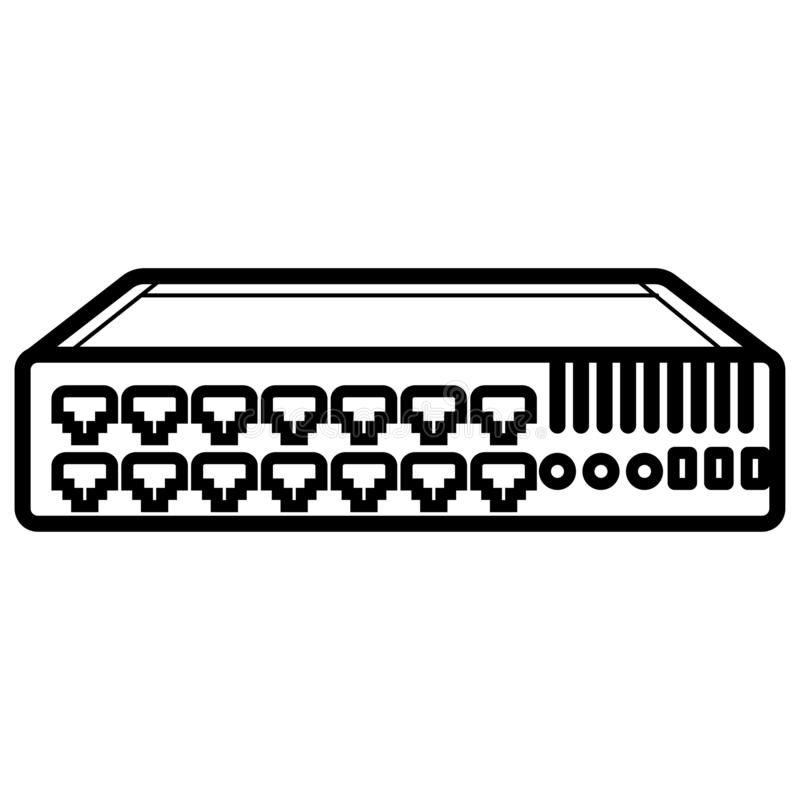
\includegraphics[width=1cm]{images/switch.jpg}};
            \node at (90:2) (b) {
\includegraphics[width=1cm]{images/computer.png}};
            \node at (-30:2) (c) {
\includegraphics[width=1cm]{images/computer.png}};
            \node at (-150:2) (d) {
\includegraphics[width=1cm]{images/computer.png}};
            \draw[dashed,very thick] (a) -- (b) (a) -- (c) (a) -- (d);
        \end{tikzpicture}
        \caption{A switched network.}
        \label{fig:switched}
    \end{subfigure}
    \caption{}
\end{figure}

In a star topology, the central device places an important and unique role. For this reason, it is very often replaced with a specialized network device called a switch. We will discuss switches in the following section.

\subsection{Switches}

A \emph{switch} is a device dedicated to moving packets through a network. It is designed to play the role of the central device in the star topology in Figure \ref{fig:star}. A typical switch may have dozens of Ethernet ports used to connect devices to it. The switch can receive packets from devices through these ports, and knows how to read the destination address of each packet. It forwards every packet along the cable pointing to the destination address, and nowhere else. This way, an Ethernet cable connected to a device is only every carrying packets sent from that device or intended for that device. A switched network is depicted in Figure \ref{fig:switched}.

It is useful to think about a switch in terms of the network layers we covered in Section \ref{sec:network:layers}. A switch is typically an Internet layer device. The Internet layer runs on top of the link layer, and so switches have link layer technology as well: these are the Ethernet ports and cables which allow devices to connect. Once a packet arrives at the switch, it uses the IP protocol in order to forward that packet to the appropriate device on the network. The flow of data from device to device follows the pattern in Figure \ref{fig:switch_layers}.

\begin{figure}
    \centering
    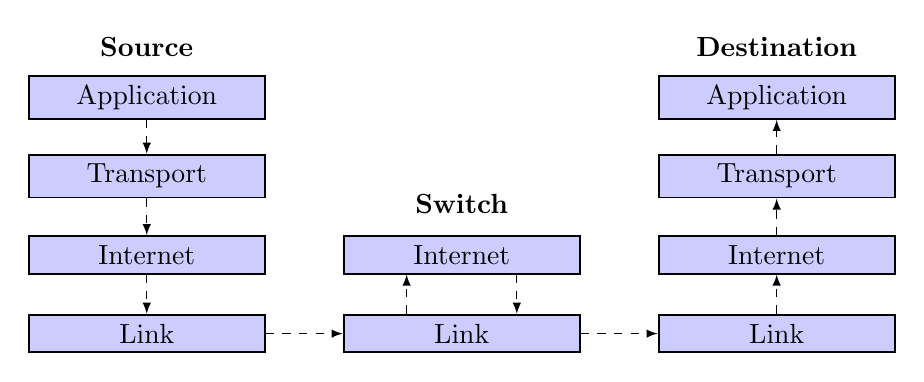
\begin{tikzpicture}[layer/.style={fill=blue!20,minimum width=3cm,align=center,text width=2.5cm,draw=black,solid,line width=.25mm},yscale=0.5]
        \node[above] at (-4, 4.8) {\textbf{Source}};
        \node[layer] at (-4, 4) (a1) {Application};
        \node[layer] at (-4, 2) (a2) {Transport};
        \node[layer] at (-4, 0) (a3) {Internet};
        \node[layer] at (-4, -2) (a4) {Link};

        \node[above] at (0, 0.8) {\textbf{Switch}};
        \node[layer] at (0, 0) (b1) {Internet};
        \node[layer] at (0, -2) (b2) {Link};

        \node[above] at (4, 4.8) {\textbf{Destination}};
        \node[layer] at (4, 4) (c1) {Application};
        \node[layer] at (4, 2) (c2) {Transport};
        \node[layer] at (4, 0) (c3) {Internet};
        \node[layer] at (4, -2) (c4) {Link};

        \draw[dashed,-latex] (a1) -- (a2);
        \draw[dashed,-latex] (a2) -- (a3);
        \draw[dashed,-latex] (a3) -- (a4);
        \draw[dashed,-latex] (a4) -- (b2);
        \draw[dashed,-latex,transform canvas={xshift=-.7cm}] (b2) -- (b1);
        \draw[dashed,-latex,transform canvas={xshift=.7cm}] (b1) -- (b2);
        \draw[dashed,-latex] (b2) -- (c4);
        \draw[dashed,-latex] (c4) -- (c3);
        \draw[dashed,-latex] (c3) -- (c2);
        \draw[dashed,-latex] (c2) -- (c1);
    \end{tikzpicture}
    \caption{The flow of data through network layers in a switched network.}
    \label{fig:switch_layers}
\end{figure}

Imagine a LAN with 50 devices connected to a switch. There are over a thousand different pairs of devices which may need to communicate with another, and the switch enables them to all communicate as if they had a dedicated cable between them, while actually using only 50 cables. This is the essential feature of any network: with relatively few physical connections, they enable an enormous number of potential communication channels. The Internet at large is designed in roughly the same way. We will discuss the details of the organization of the Internet, or more generally any wide area network, in the following section.

\section{Wide Area Networks}

Almost every LAN needs a way of communicating with the outside world. A network at a larger scale than a LAN is called a Wide Area Network (WAN). By far the most familiar example of a WAN is the Internet, but a WAN need not be this large. For example, a campus or metropolitan area may have its network organized as a WAN.

The link layer technology which carries signals over a WAN is similar to that of a LAN. A WAN typically needs higher capacity Ethernet cables, but the general principles are the same. The primary difference between a LAN and a WAN comes in at the Internet layer, where the IP protocol distinguishes between public and private networks. In this section we will discuss this difference, and the systems and protocols used to connect public networks together.

\subsection{Gateways and Routing}

If you have used a home network, you may be more familiar with routers than switches. This is because a switch is designed to connect all the devices into an area into a local network, but typically we also want to connect a local network to the outside Internet. This is the role of a router. Routers are responsible for connecting different networks together into a larger network.

In a typical setup, several devices on a local network will be connected to a router. The router assigns private IP addresses to each of these devices. Private IP addresses belong to one of three special blocks reserved for this purpose. The most common block is 192.168.*.*, any address ranging from 192.168.0.0 to 192.168.255.255. There are about 65,000 such addresses. A block like this can be written as 192.168.0.0/16, meaning the first 16 bits are fixed and the rest can change. The other private IP address blocks are 172.16.0.0/12, with about 1 million addresses, and 10.0.0.0/8, with about 16 million addresses.

When a device (such as a switch) within a LAN receives a packet, it will look at the destination IP address. If the packet is destined for another device on the LAN, then the switch will forward the packet appropriately. If the switch does not know where to route the packet, then it will forward the packet to a device designated as the \emph{default gateway} for the network. The default gateway is typically the router.

When the router receives a packet with a destination address outside of the LAN, it will forward the packet appropriately, using the following steps. First, the router will change the source address of the packet. The packet originated from a device on the private network, so its source address is a private address, such as 192.168.1.4. The router will replace this source address with its own address on the WAN. This will be a public IP address, such as 172.217.15.100. Next, the router sends the packet out to the public Internet and awaits a reply. When the router receives a reply, it will forward the packet on to the correct device on the network. This process is depicted in Figure \ref{fig:gateway}. 

\begin{figure}
    \centering
    \begin{tikzpicture}
        \useasboundingbox (-8,-1.5) rectangle (5,2.5);
        \begin{scope}[transform canvas={scale=.8}]
        \node[label={[align=center]90:Private: 192.168.1.1\\Public: 172.217.15.100}] at (0,0) (a) {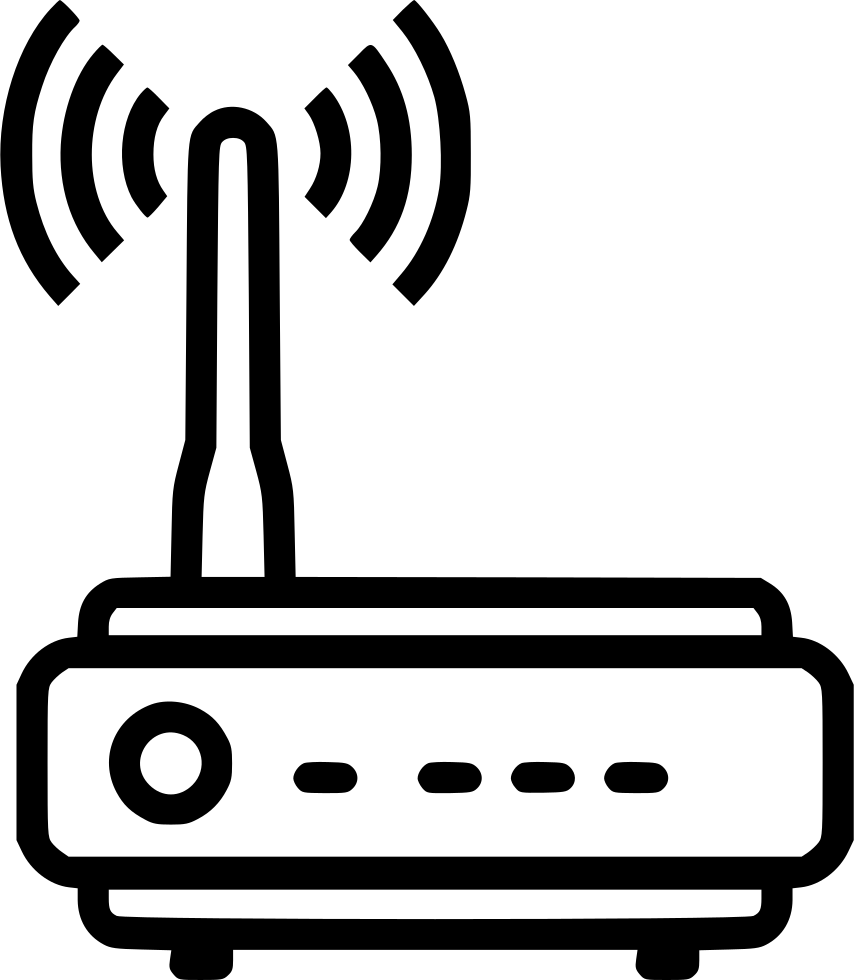
\includegraphics[width=1cm]{images/router.png}};
        \node[label={180:192.168.1.2}] at (-5,2) (b) {
\includegraphics[width=1cm]{images/computer.png}};
        \node[label=180:{192.168.1.3}] at (-6,1) (c) {
\includegraphics[width=1cm]{images/computer.png}};
        \node[label=180:{192.168.1.4}] at (-7,0) (d) {
\includegraphics[width=1cm]{images/computer.png}};
        \draw[dashed,very thick] (b) -- (a) (c) -- (a) (d) -- (a);
        \node[draw,thick,right,align=left] at (-6,-0.7) (packet) {\scriptsize Source: 192.168.1.4\\\scriptsize Destination: 208.80.153.224};
        \draw[thick,->] (packet) -- (-1.5,-0.7);
        \node[draw,thick,right,align=left] at (2,-0.7) (packet2) {\scriptsize Source: 172.217.15.100\\\scriptsize Destination: 208.80.153.224};
        \draw[thick,->] (1,-0.7) -- (packet2);
        \draw[dashed,very thick] (a) -- ++(5,0) node[above left] (cloud) {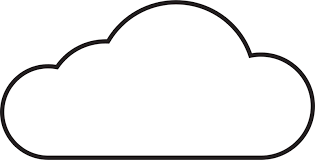
\includegraphics[width=2cm]{images/cloud.png}};
        \node at (cloud) {Internet};
        \end{scope}
    \end{tikzpicture}
    \caption{The default gateway forwards packets from a LAN to a WAN.}
    \label{fig:gateway}
\end{figure}

\subsection{Autonomous Systems}

Once a packet is routed to the Internet, it needs to be sent to the network which contains the destination address. Typically, the first destination for a packet is a router belonging to an Internet Service Provider (ISP). For example, in the \ic{traceroute} trace on page \pageref{code:traceroute}, the packet ends up at a router owned by Verizon, a popular ISP. This router belongs to an \emph{autonomous system} (AS) operated by Verizon. An autonomous system is simply a connection of routers on the Internet which are under common administrative control (e.g. the ISP).

Autonomous systems are managed globally using autonomous system numbers, or ASNs, which are similar to IP addresses. These numbers are allocated by the Internet Assigned Numbers Authority (IANA) to Regional Internet Registries (RIRs), which then assign the numbers to autonomous systems.

The routers in an autonomous system can forward packets to destinations within the same AS, but if a packet is destined for a network on another AS, it needs to be routed appropriately. This requires different AS's to communicate with one another. This can happen via \emph{peering}, in which two AS's mutually agree to carry traffic to one another free of charge, or via \emph{transit}, in which an AS charges a fee to carry traffic from other AS's.

When two ASs need to communicate with one another, they use the Border Gateway Protocol (BGP). This is the core routing protocol of the Internet, and is responsible for making decisions on how to get packets to a destination in the quickest way possible. 

\exercisesection

\begin{exercise}
    What is the difference between a switch and a router? On which type of network would each be used?
\end{exercise}

\begin{exercise}
    Margaret has been hired as a network administrator to set up a network for Acme, Inc. Acme has 10 computers in their office, and there is no network in place. If Margaret wants to put a unique cable between every pair of computers, how many cables will she need? 
    %If Margaret wants to use the minimum number of cables to ensure every computer has a path in the network to every other computer, how many cables will she need?
\end{exercise}

\begin{exercise}
    What do ISP and AS stand for? What is the relationship between an ISP and an AS?
    %If Margaret wants to use the minimum number of cables to ensure every computer has a path in the network to every other computer, how many cables will she need?
\end{exercise}

\begin{exercise}
    What do LAN and WAN stand for? What is the relationship between a LAN and a WAN?
\end{exercise}